\documentclass[aspectratio=1610]{beamer}

\usepackage[ngerman]{babel}
\usepackage[utf8]{inputenc}
\usepackage[absolute,overlay]{textpos}
\usepackage{xcolor}
\usepackage{hyperref}
\usetheme{lankton-keynote}

\newcommand{\concept}[2]{
  \begin{block}{#1}
    \pause
    #2
  \end{block}
}

\newcommand{\pattern}[2]{
  \begin{alertblock}{Problem}
    #1
  \end{alertblock}
  \pause
  \begin{exampleblock}{Lösung}
    #2
  \end{exampleblock}
}

\newcommand{\boxx}[1]{
  \colorbox{black}{
    \color{gray}{#1}
  }
}

\newcommand{\photoby}[3]{
  \begin{textblock*}{\paperwidth}[0.15,0](\textwidth,\textheight)
    \raggedright{
      \boxx{
        \tiny{
          Foto von \href{#2}{#1} (#3)
        }
      }
    }
  \end{textblock*}
}

\AtBeginSubsection[]{
  \begin{frame}
    \tableofcontents[currentsection, currentsubsection]
  \end{frame}
}

\huge

\title{Hack the Space}

\author[Mic]{Mic \flq nomaster@chaosdorf.de\frq}

\begin{document}

  \begin{frame}
    \titlepage
  \end{frame}

  \begin{frame}{Was zur \ldots?}
    \concept{Hackspace}{
      Ein \textsl{Hackspace} ist ein physischer, kollektiv betriebener Raum,\\
      in dem Menschen sich treffen können und an ihren Projekten arbeiten.\\
    }
    \pause
    \textsl{Alternative Bezeichnungen:\\Hackerspace, Makerspace, Makespace,
    Hacklab, Hackcenter.}
  \end{frame}

  {
    \usebackgroundtemplate{\includegraphics[width=\paperwidth]{hack42.jpg}}
    \begin{frame}{\boxx{Arnheim}}
      \photoby{dvanzuijlekom}{https://secure.flickr.com/photos/dv_anzuijlekom/6854225951/}{CC by-sa}
    \end{frame}
  }


  \begin{frame}{Aktivitäten}
    \begin{itemize}
      \item Do It Yourself
      \item Workshops
      \item Vorträge
      \item Teilen von Wissen
      \item Spaß haben
    \end{itemize}
  \end{frame}

  {
    \usebackgroundtemplate{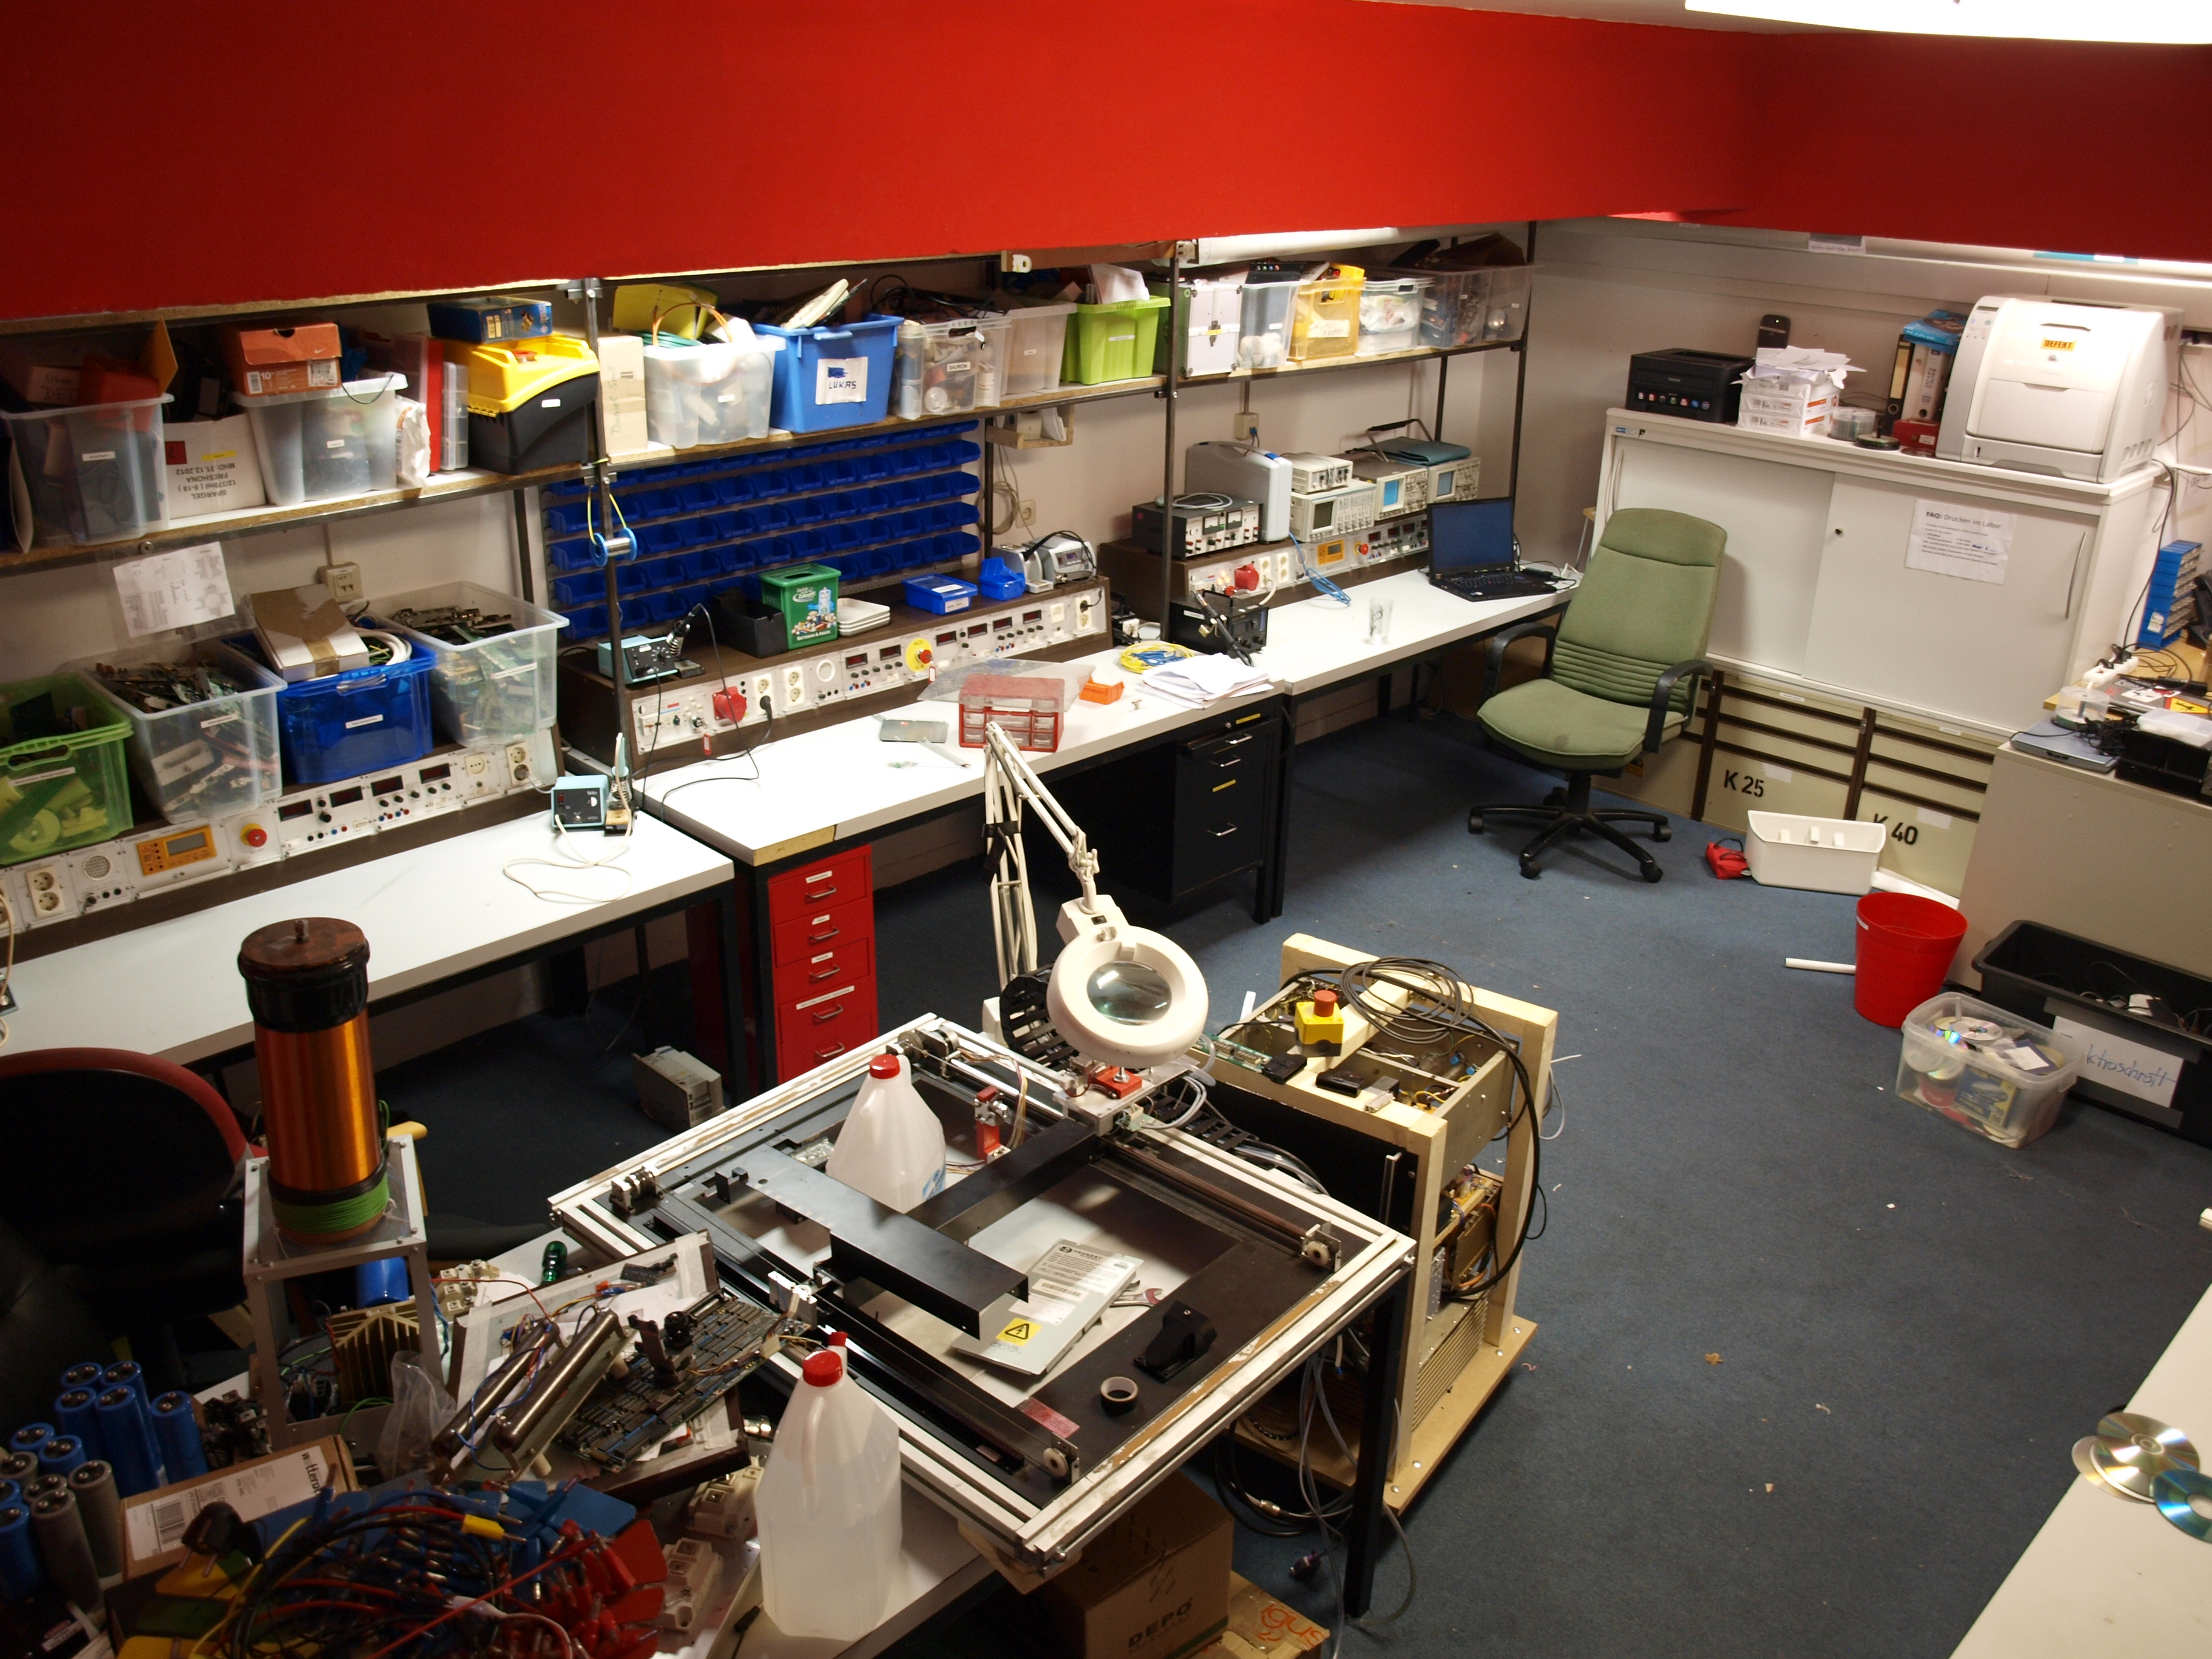
\includegraphics[width=\paperwidth]{daslabor.jpg}}
    \begin{frame}{\boxx{Bochum}}
      \photoby{Das Labor}{http://das-labor.org/wiki/Datei:Bastelraum\_1.JPG}{GNU FDL}
    \end{frame}
  }

   \begin{frame}{Infrastruktur}
    \begin{itemize}
      \item Strom
      \item Computer-Netzwerk
      \item Internetzugang
      \item Werkzeuge und Maschinen
      \item Getränke
    \end{itemize}
  \end{frame}

  {
    \usebackgroundtemplate{\includegraphics[width=\paperwidth]{infrastructure.jpg}}
    \begin{frame}{\boxx{Milwaukee}}
      \photoby{dreamexplorer}{https://secure.flickr.com/photos/dreamexplorer/5739464898/}{CC by-nc-sa}
    \end{frame}
  }

   \begin{frame}{Rules}
    \begin{itemize}
      \item Be excellent to each other!\footnote{Die einzige echte Regel}
      \item Mache dich nicht abhängig
      \item Erforsche die Welt
      \item Entdecke dich selbst
    \end{itemize}
   \end{frame}
 {
    \usebackgroundtemplate{\includegraphics[width=\paperwidth]{noisebridge.jpg}}
    \begin{frame}{\boxx{San Francisco}}
      \photoby{maltman23}{https://secure.flickr.com/photos/maltman23/6254785979/}{CC by-sa}
    \end{frame}
  }

  {
    \usebackgroundtemplate{\includegraphics[width=\paperwidth]{coziness.jpg}}
    \begin{frame}{\boxx{New York City}}
      \photoby{girl\_onthe\_les}{https://secure.flickr.com/photos/girlontheles/6164704739/}{CC by-nc-nd}
    \end{frame}
  }

  {
    \usebackgroundtemplate{\includegraphics[width=\paperwidth]{talk.jpg}}
    \begin{frame}{\boxx{Sidney}}
      \photoby{Alegrya}{https://secure.flickr.com/photos/alegrya/3670712239/}{CC by-nc-sa}
    \end{frame}
  }

  {
    \usebackgroundtemplate{\includegraphics[width=\paperwidth]{bike-rack.jpg}}
    \begin{frame}{\boxx{Detroit}}
      \photoby{Bradmcmahon}{https://secure.flickr.com/photos/bradmcmahon/5388909742/}{CC by-nc}
    \end{frame}
  }

  {
    \usebackgroundtemplate{\includegraphics[width=\paperwidth]{stgo.jpg}}
    \begin{frame}{\boxx{Santiago de Chile}}
      \photoby{maltman23}{https://secure.flickr.com/photos/maltman23/9730117045/}{CC by-nc}
    \end{frame}
  }

 {
    \usebackgroundtemplate{\includegraphics[width=\paperwidth]{ps-one.jpg}}
    \begin{frame}{\boxx{Chicago}}
      \photoby{opacity}{https://secure.flickr.com/photos/opacity/402846170}{CC by-nc-sa}
    \end{frame}
  }

  {
    \usebackgroundtemplate{\includegraphics[width=\paperwidth]{makerfaire-africa.jpg}}
    \begin{frame}{\boxx{Cairo}}
      \photoby{maltman23}{https://secure.flickr.com/photos/maltman23/9730117045/}{CC by-nc}
    \end{frame}
  }

  {
    \usebackgroundtemplate{\includegraphics[width=\paperwidth]{ohm.jpg}}
    \begin{frame}{\boxx{\#OHM2013}}
      \photoby{nuridao}{https://secure.flickr.com/photos/nuridao/9458063039}{CC by-nc-sa}
    \end{frame}
  }
  {
    \usebackgroundtemplate{\includegraphics[width=\paperwidth]{ideas.jpg}}
    \begin{frame}
      \photoby{seanbonner}{https://secure.flickr.com/photos/seanbonner/8180645274}{CC by-nc-sa}
    \end{frame}
  }

\end{document}
